
\subsubsection{Network Throughput}
    \begin{figure}[!h]
        \centering
        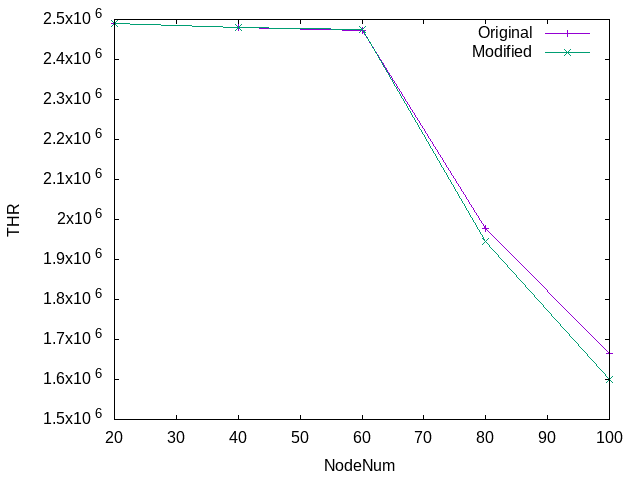
\includegraphics[width=.9\textwidth]{Pictures/Wired/Combined/THRVSNodeNum.png}
        \caption{Wired : Network Throughput VS Number of Nodes}
    \end{figure}
    
     \begin{figure}[!h]
        \centering
        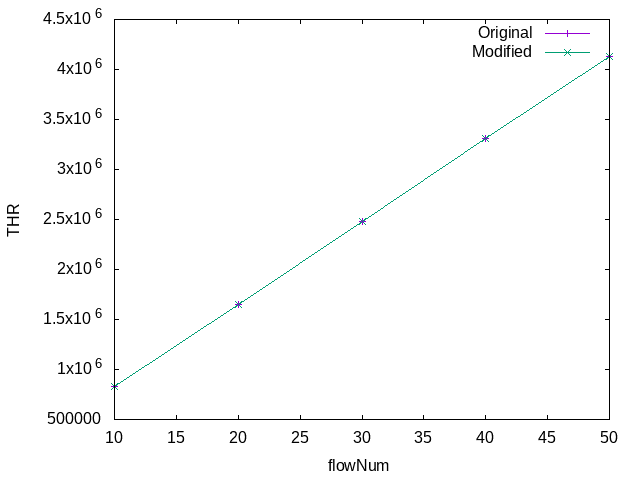
\includegraphics[width=.9\textwidth]{Pictures/Wired/Combined/THRVSflowNum.png}
        \caption{Wired : Network Throughput VS Number of Flows}
    \end{figure}
    
    \begin{figure}[!h]
        \centering
        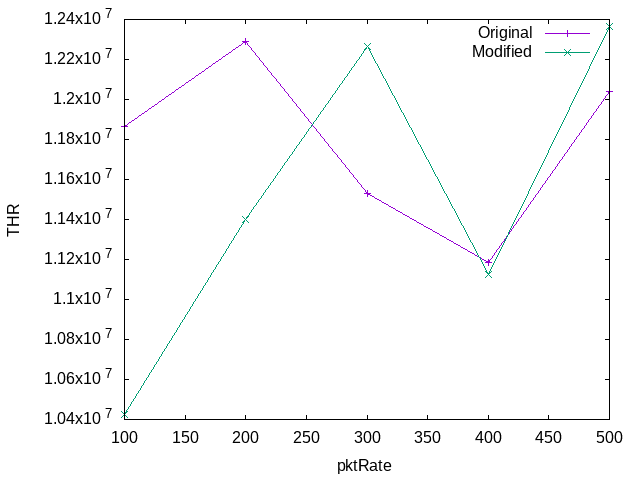
\includegraphics[width=.9\textwidth]{Pictures/Wired/Combined/THRVSpktRate.png}
        \caption{Wired : Network Throughput VS Packets Per Second}
    \end{figure}
    

\newpage
\subsubsection{End-to-End Delay}
    \begin{figure}[!h]
        \centering
        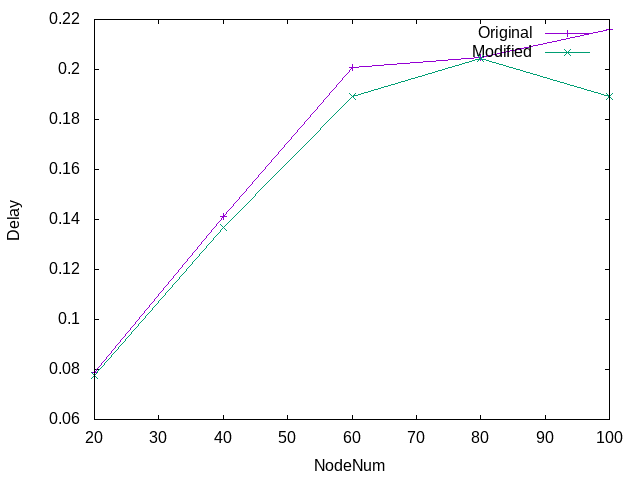
\includegraphics[width=.9\textwidth]{Pictures/Wired/Combined/DelayVSNodeNum.png}
        \caption{Wired : Delay VS Number of Nodes}
    \end{figure}
    
     \begin{figure}[!h]
        \centering
        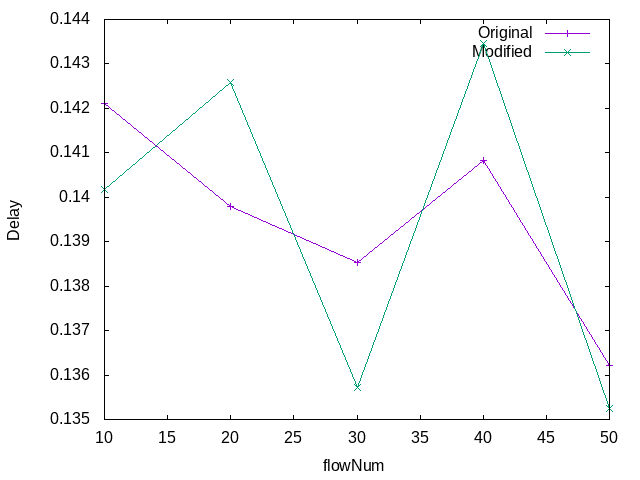
\includegraphics[width=.9\textwidth]{Pictures/Wired/Combined/DelayVSflowNum.png}
        \caption{Wired : Delay VS Number of Flows}
    \end{figure}
    
    \begin{figure}[!h]
        \centering
        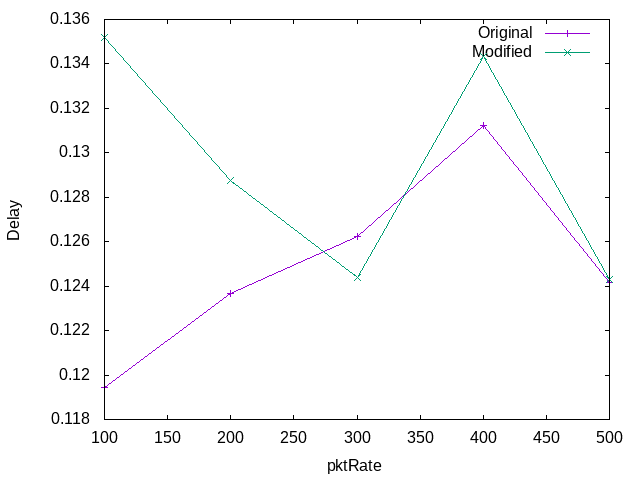
\includegraphics[width=.9\textwidth]{Pictures/Wired/Combined/DelayVSpktRate.png}
        \caption{Wired : Delay VS Packets Per Second}
    \end{figure}
    
\newpage
\subsubsection{Packet Delivery Ratio}
    \begin{figure}[!h]
        \centering
        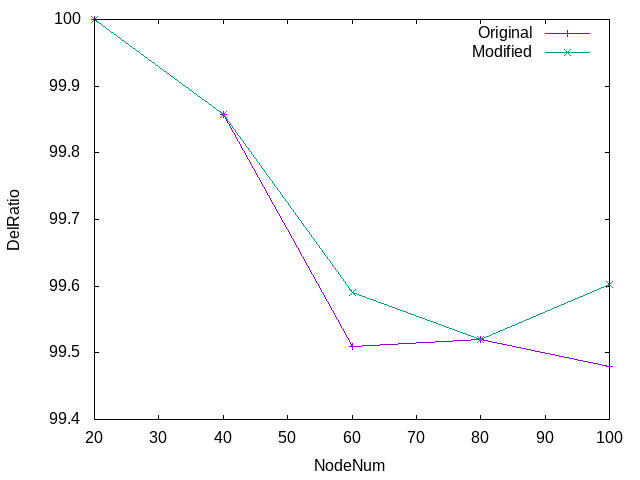
\includegraphics[width=.9\textwidth]{Pictures/Wired/Combined/DelRatioVSNodeNum.png}
        \caption{Wired : Delivery Ratio VS Number of Nodes}
    \end{figure}
    
     \begin{figure}[!h]
        \centering
        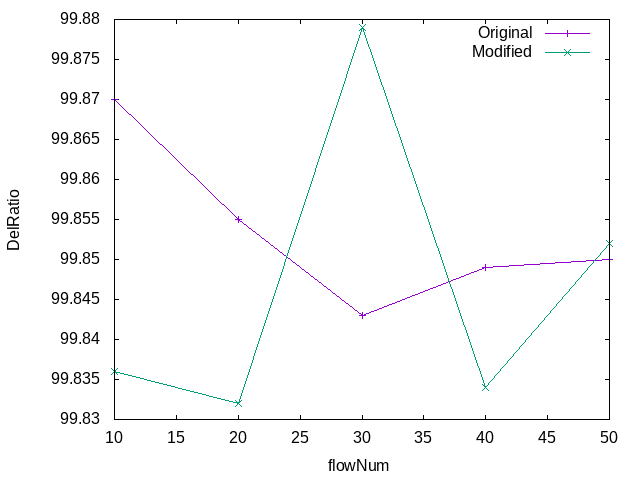
\includegraphics[width=.9\textwidth]{Pictures/Wired/Combined/DelRatioVSflowNum.png}
        \caption{Wired : Delivery Ratio VS Number of Flows}
    \end{figure}
    
    \begin{figure}[!h]
        \centering
        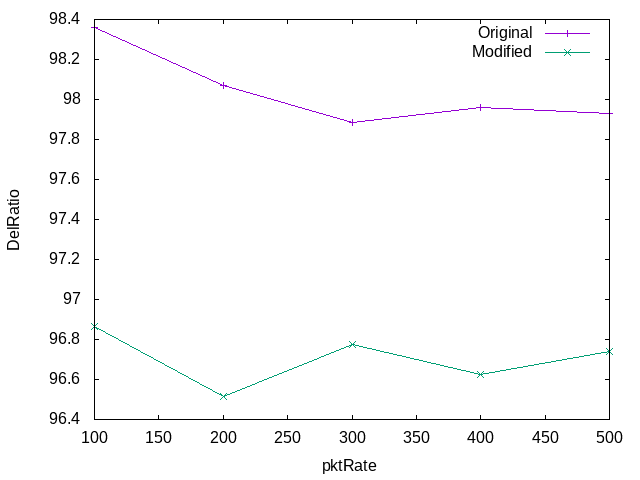
\includegraphics[width=.9\textwidth]{Pictures/Wired/Combined/DelRatioVSpktRate.png}
        \caption{Wired : Delivery Ratio VS Packets Per Second}
    \end{figure}

\newpage
\subsubsection{Packet Drop Ratio}
    \begin{figure}[!h]
        \centering
        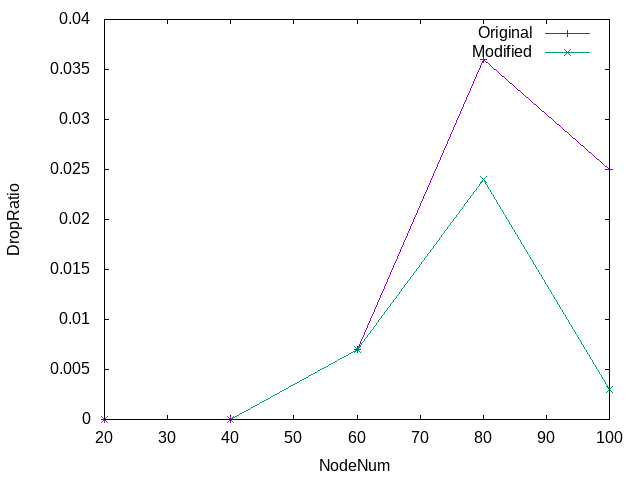
\includegraphics[width=.9\textwidth]{Pictures/Wired/Combined/DropRatioVSNodeNum.png}
        \caption{Wired : Drop Ratio VS Number of Nodes}
    \end{figure}
    
     \begin{figure}[!h]
        \centering
        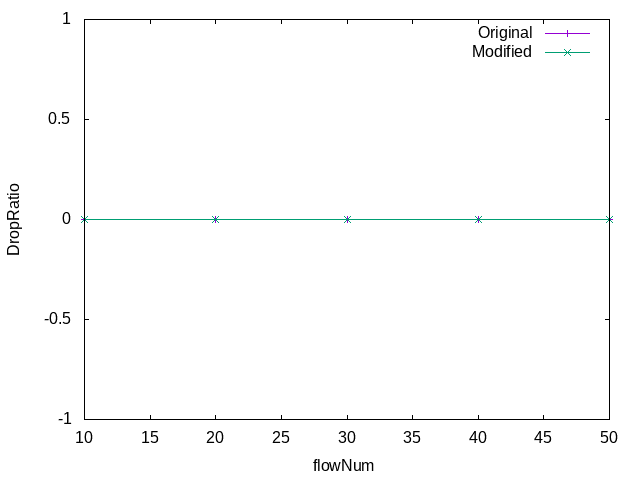
\includegraphics[width=.9\textwidth]{Pictures/Wired/Combined/DropRatioVSflowNum.png}
        \caption{Wired : Drop Ratio VS Number of Flows}
    \end{figure}
    
    \begin{figure}[!h] 
        \centering
        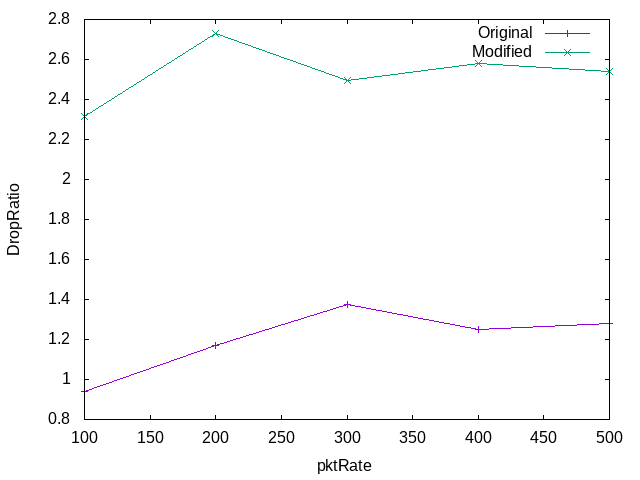
\includegraphics[width=.9\textwidth]{Pictures/Wired/Combined/DropRatioVSpktRate.png}
        \caption{Wired : Drop Ratio VS Packets Per Second}
    \end{figure}
    
\newpage
\subsubsection{Average Congestion Window}
    
    \begin{figure}[!h]
    	\centering
    	
    	\begin{subfigure}{0.9\textwidth}[!h] % width of left subfigure
    		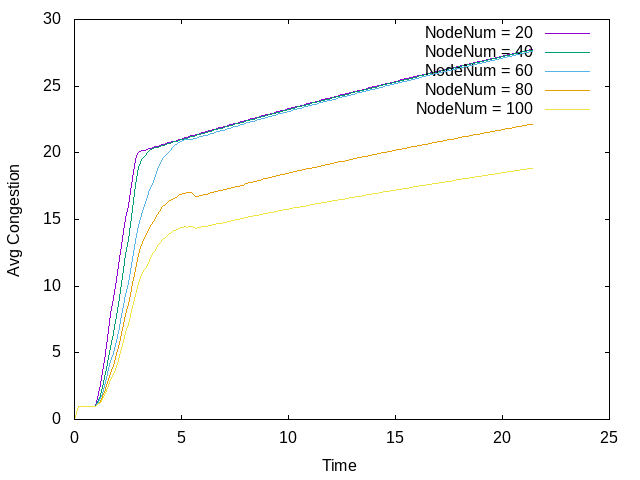
\includegraphics[width=.95\textwidth]{Pictures/Wired/Original/Avg_CongestionVSNodeNum.png}
    		\caption{Original} % subcaption
    	\end{subfigure}
    	
    	\vspace{1em} % here you can insert horizontal or vertical space
    	
    	\begin{subfigure}{0.9\textwidth}[!h] % width of left subfigure
    		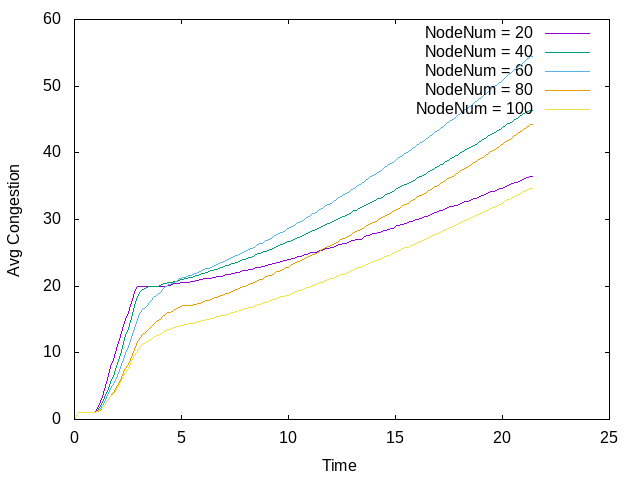
\includegraphics[width=.95\textwidth]{Pictures/Wired/Modified/Avg_CongestionVSNodeNum.png}
    		\caption{Modified} % subcaption
    	\end{subfigure}
    	
    	\caption{Wired : Average Congestion Window VS Number of Nodes} % caption for whole figure
    \end{figure}
    
    \begin{figure}[!h]
    	\centering
    	
    	\begin{subfigure}{0.9\textwidth}[!h] % width of left subfigure
    		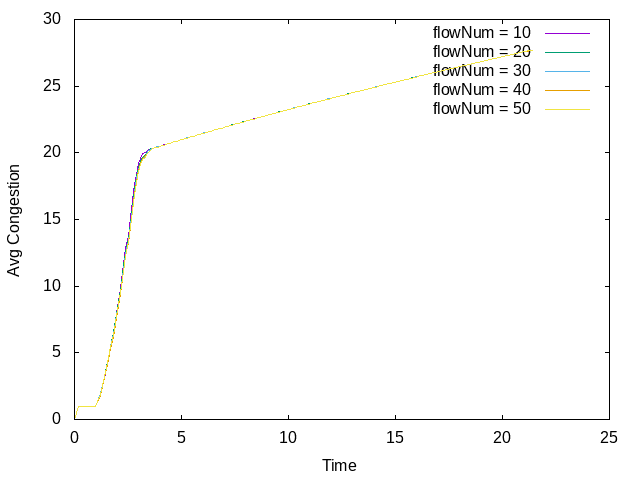
\includegraphics[width=.95\textwidth]{Pictures/Wired/Original/Avg_CongestionVSflowNum.png}
    		\caption{Original} % subcaption
    	\end{subfigure}
    	
    	\vspace{1em} % here you can insert horizontal or vertical space
    	
    	\begin{subfigure}{0.9\textwidth}[!h] % width of left subfigure
    		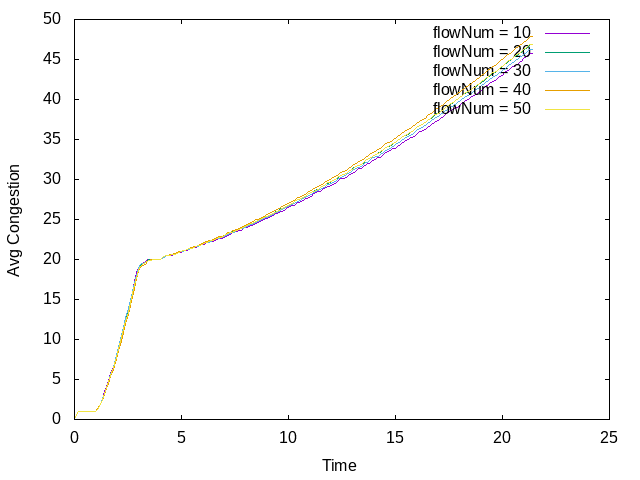
\includegraphics[width=.95\textwidth]{Pictures/Wired/Modified/Avg_CongestionVSflowNum.png}
    		\caption{Modified} % subcaption
    	\end{subfigure}
    	
    	\caption{Wired : Average Congestion Window VS Number of Flows} % caption for whole figure
    \end{figure}
    
    \begin{figure}[!h]
    	\centering
    	
    	\begin{subfigure}{0.9\textwidth}[!h] % width of left subfigure
    		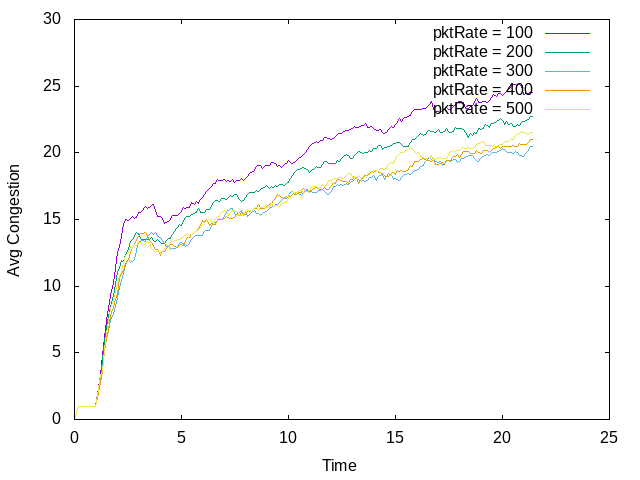
\includegraphics[width=.95\textwidth]{Pictures/Wired/Original/Avg_CongestionVSpktRate.png}
    		\caption{Original} % subcaption
    	\end{subfigure}
    	
    	\vspace{1em} % here you can insert horizontal or vertical space
    	
    	\begin{subfigure}{0.9\textwidth}[!h] % width of left subfigure
    		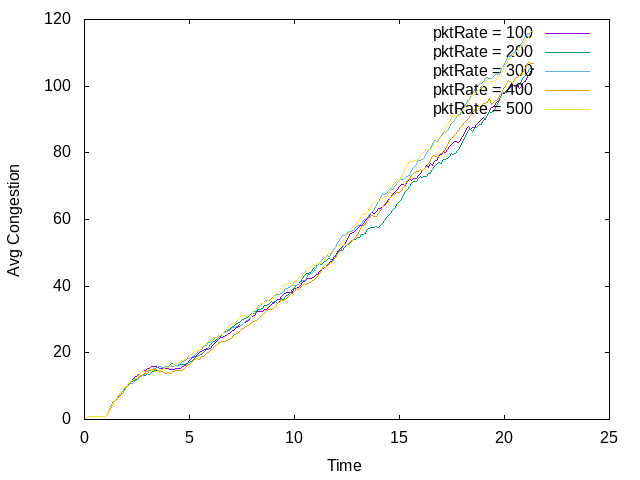
\includegraphics[width=.95\textwidth]{Pictures/Wired/Modified/Avg_CongestionVSpktRate.png}
    		\caption{Modified} % subcaption
    	\end{subfigure}
    	
    	\caption{Wired : Average Congestion Window VS Packets Per Seconds} % caption for whole figure
    \end{figure}

\vspace{1cm}
    
\newpage
\subsubsection{Per-Node Throughput}
    
    \begin{figure}[!h]
    	\centering
    	
    	\begin{subfigure}{0.9\textwidth}[!h] % width of left subfigure
    		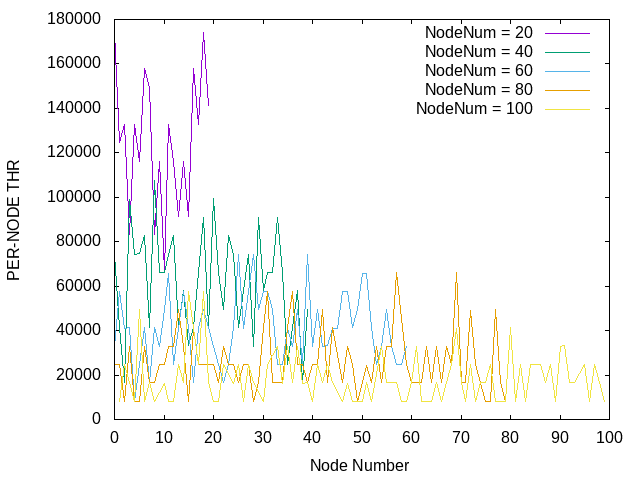
\includegraphics[width=.95\textwidth]{Pictures/Wired/Original/PER-NODETHRVSNodeNum.png}
    		\caption{Original} % subcaption
    	\end{subfigure}
    	
    	\vspace{1em} % here you can insert horizontal or vertical space
    	
    	\begin{subfigure}{0.9\textwidth}[!h] % width of left subfigure
    		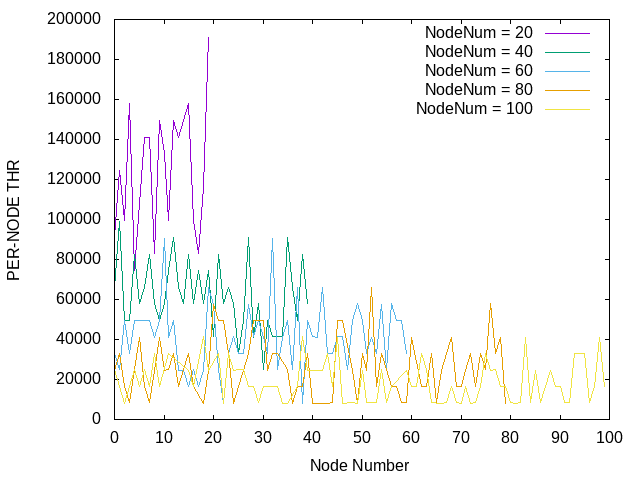
\includegraphics[width=.95\textwidth]{Pictures/Wired/Modified/PER-NODETHRVSNodeNum.png}
    		\caption{Modified} % subcaption
    	\end{subfigure}
    	
    	\caption{Wired : Per-Node Throughput VS Number of Nodes} % caption for whole figure
    \end{figure}
    
    \begin{figure}[!h]
    	\centering
    	
    	\begin{subfigure}{0.9\textwidth}[!h] % width of left subfigure
    		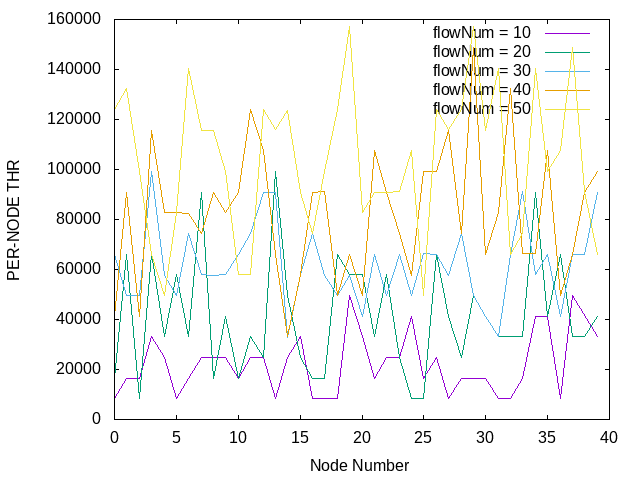
\includegraphics[width=.95\textwidth]{Pictures/Wired/Original/PER-NODETHRVSflowNum.png}
    		\caption{Original} % subcaption
    	\end{subfigure}
    	
    	\vspace{1em} % here you can insert horizontal or vertical space
    	
    	\begin{subfigure}{0.9\textwidth}[!h] % width of left subfigure
    		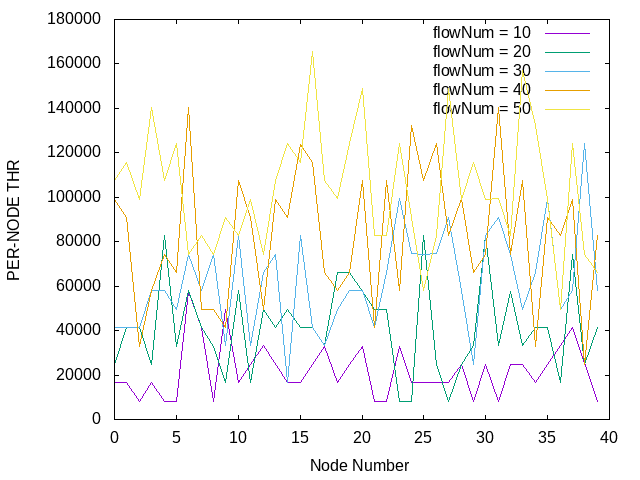
\includegraphics[width=.95\textwidth]{Pictures/Wired/Modified/PER-NODETHRVSflowNum.png}
    		\caption{Modified} % subcaption
    	\end{subfigure}
    	
    	\caption{Wired : Per-Node Throughput VS Number of Flows} % caption for whole figure
    \end{figure}
    
    \begin{figure}[!h]
    	\centering
    	
    	\begin{subfigure}{0.9\textwidth}[!h] % width of left subfigure
    		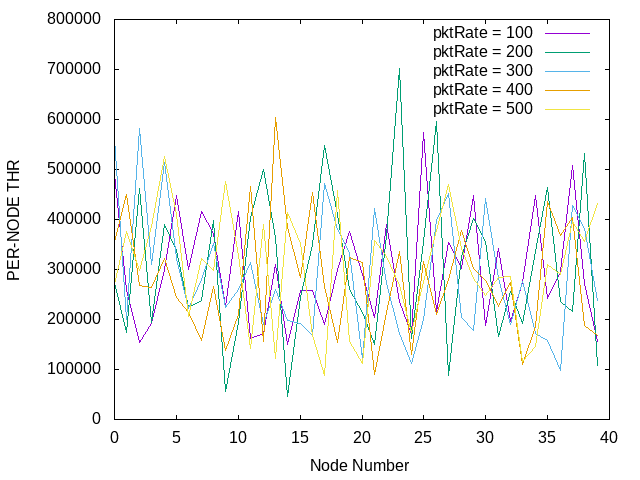
\includegraphics[width=.95\textwidth]{Pictures/Wired/Original/PER-NODETHRVSpktRate.png}
    		\caption{Original} % subcaption
    	\end{subfigure}
    	
    	\vspace{1em} % here you can insert horizontal or vertical space
    	
    	\begin{subfigure}{0.9\textwidth}[!h] % width of left subfigure
    		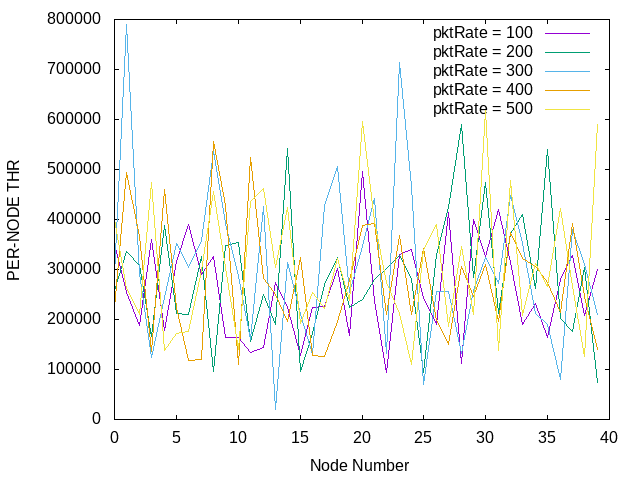
\includegraphics[width=.95\textwidth]{Pictures/Wired/Modified/PER-NODETHRVSpktRate.png}
    		\caption{Modified} % subcaption
    	\end{subfigure}
    	
    	\caption{Wired : Per-Node Throughput VS Packets Per Seconds} % caption for whole figure
    \end{figure}

    